\section{Experiment Design}
\label{sec:experiment}

This section describes the experiment design. The study was approved by the university's Institutional Review Board (IRB). 

\subsection{Participant Recruitment}
This study recruited 202 Amazon Mechanical Turk (MTurk) participants using stratified sampling. The system screened participants based on their age, gender, household income, and education level to assure a balanced demographic within each experiment condition while randomly assigning participants to these conditions. This approach aimed to mitigate imbalanced participation demographics~\cite{redmilesHowWellMy2019}. We provide the demographic in Table X?

\begin{figure}[t]
    \centering
    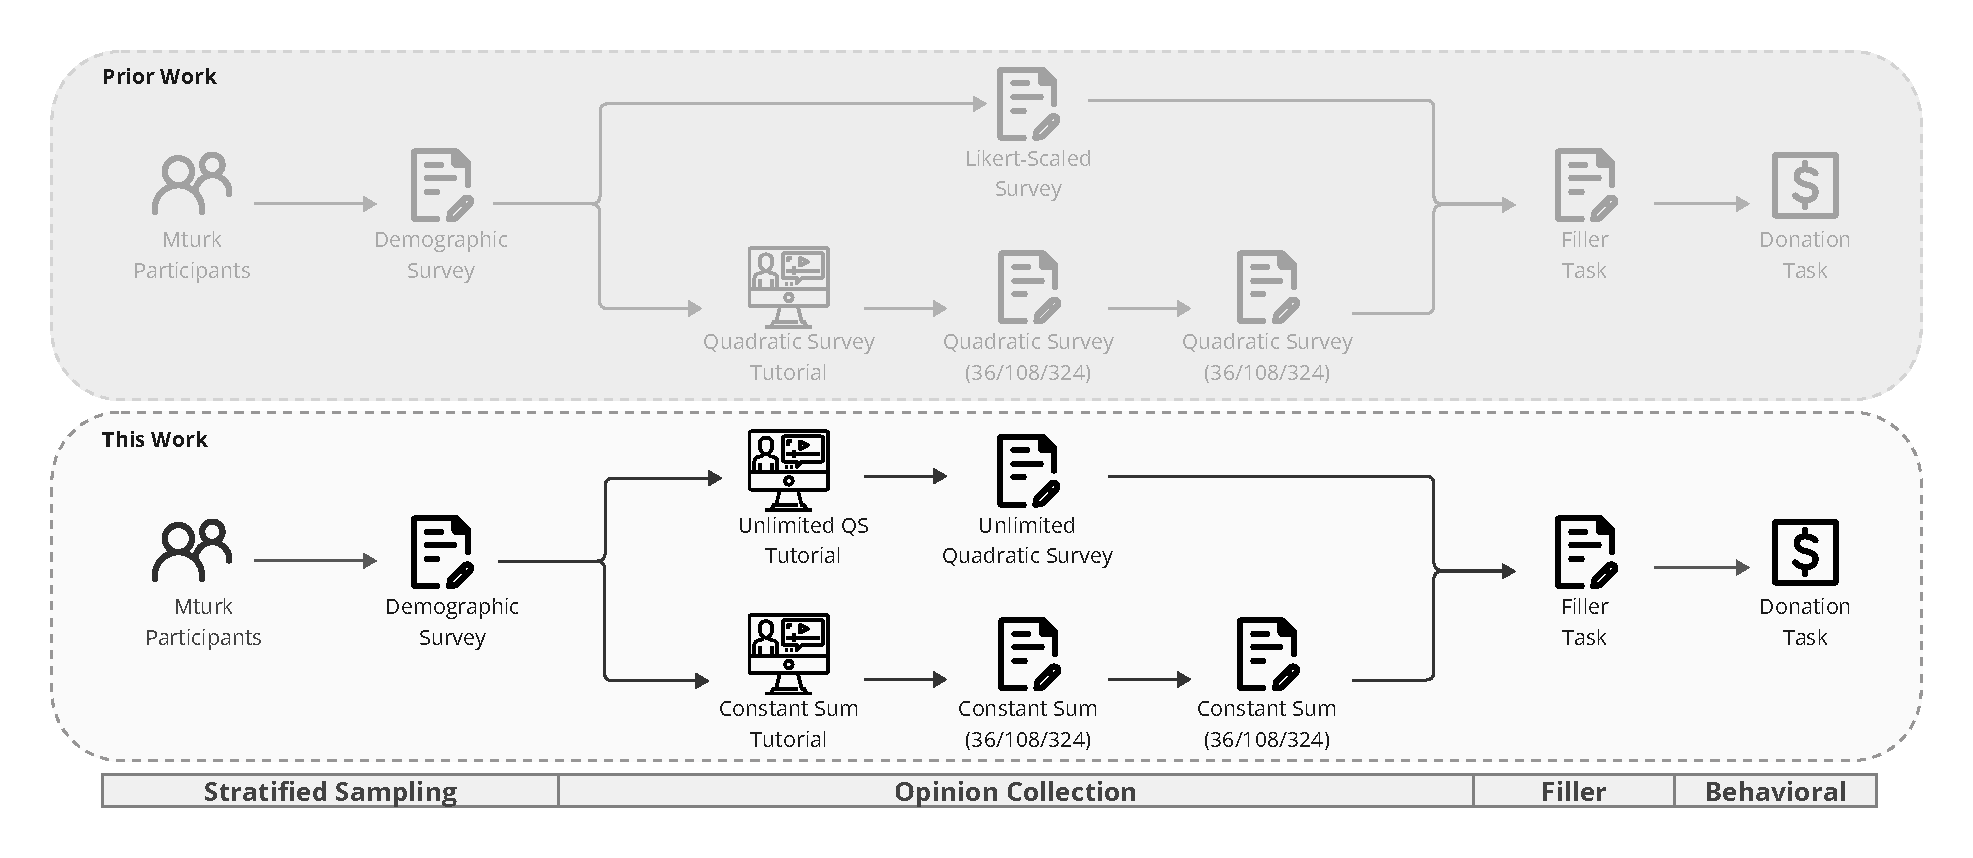
\includegraphics[width=\textwidth]{content/image/whyqs_exp_flow.pdf}
    \caption{Experiment overview. Our study covers the dotted box beneath, mirroring prior research only differing the type of surveys involved during the opinion collection section. The bar below highlights the four parts of the study: sampling, opinion collection, filler task, and the behavioral task.}
    \label{fig:experiment}
\end{figure}

\subsection{Experiment Design}
To ensure comparable data with prior study~\cite{chengCanShowWhat2021}, this study followed the same between-subject experimental design and altered the open sourced software to create two more conditions, creating four new experimental data. Refer to prior studies for details on the procedure justification of the experiment. We highlight key procedures and alternations we made to the methodology below. Figure~\ref{fig:experiment} shows how our study fits into the prior work and the overall experiment flow.

\paragraph{Additional Experimental Conditions}
We added four additional experimental conditions presented as two groups, Unlimited QS or the Constant Sum Survey (CSS) group. The CSS group was further divided into three conditions with different budgets:

\begin{itemize}
    \item **Unlimited QS (UQS):** Participants experience quadratic costs without budget constraints, isolating the effect of cost scaling.
    \item **Constant Sum Survey with 36 Credits (CS36):** A small-budget linear-cost condition testing the effect of budget constraints.
    \item **Constant Sum Survey with 108 Credits (CS108):** A medium-budget version allowing greater expressiveness.
    \item **Constant Sum Survey with 324 Credits (CS324):** A high-budget condition assessing whether increased budgets improve alignment.
\end{itemize}

The UQS condition isolates the effect of quadratic costs, while the CSS conditions isolate the effect of budget constraints. Together, these conditions allow for a direct comparison of cost mechanisms in preference elicitation. As mentioned in~\Cref{sec:related_works_css}, QS with linear cost function is slightly different then CSS where participants do not need to allocate all their provided credits, however, that effectively equals to an additional ``no response'' option on CSS, thus, here we denote these variations as CSS.

Participants assigned to the CSS completed two randomly selected CSS conditions. <report completion time>.

\subsubsection{Survey content}
The study frames the survey as a public resource allotment task, where participants express preferences across 9 societal issues such as education, environment, or health~\footnote{See supplumentary material for the full survey}. Participants would express their degree of preferences in number of votes, positive or negatively under the mechanism of UQS or CSS.

\subsubsection{Surveying process and interface}
Participants in both groups were first introduced to the survey and how to use it via a video tutoiral that we recorded. To assure their understanding of these mechanism, participants were asked to complete a quiz with 5 multiple-choice questions. Participants were required to answer at least 3 questions correctly to continue with the study. We altered the questions based on the survey mechanisms.

The number of credits for the CSS mirros those in the prior study since CSS literature does not provide a clear guideline on how to set the budget with the convension that the budget should be 100. The interface for both studies are shown in~\Cref{fig:extended_interface}.

\subsubsection{Filler task and donation}
After the survey, participants completed a filler task to prevent direct association with the issues and the charities listed on the donation task page. Participants 

\subsubsection{Debrief, and Compensation}
After the study, participants have a chance to read about the study's real purpose on the debrief page. Participants were compensated with \$1.50 for their time, and they were informed that they would receive an additional \$0.50 if they completed the study.

\subsection{Quantitative Measures: Ordinal and Interval Measures}
\label{sec:quantitative_measures}
In the prior studies, the authors used cosine similiarity to measure the alignment between the participants' preferences and their behaviors. However, this measure while useful in tackling high-dimensional data, it risks errors in interpretation. For example, an alignment deemed high by cosine similarity could be due to a large difference in the angle between two vectors with completely aligned rankings compared to a low cosine similarity value that could be due to a small difference in the angle between two vectors with completely unaligned rankings. Based on prior literature in evaluating the effectiveness of CSS, many relied on seperate evaluations of both rankings and intervals between options to evaluate.

In this study, we constructed two Bayesian model to evaluate both ordinal and interval measures of participants' survey results and behaviors.

\subsubsection{Pairwise Ordinal Measures}
\label{sec:ordinal_measures}





\subsubsection{Interval Measures}
\label{sec:interval_measures}